% Created by tikzDevice version 0.12.3.1 on 2021-06-16 15:27:58
% !TEX encoding = UTF-8 Unicode
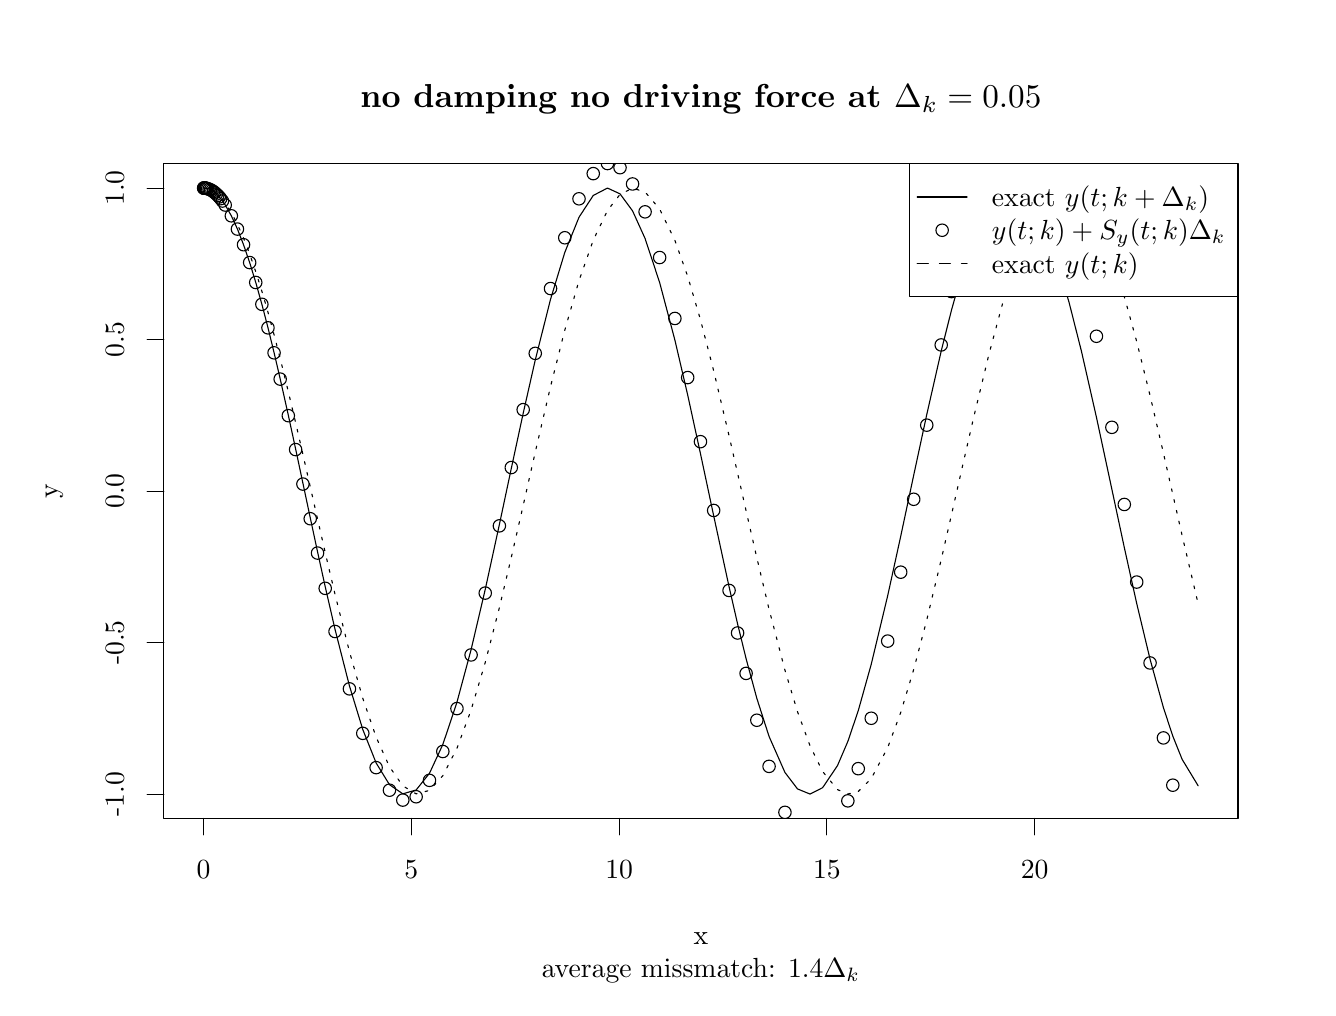
\begin{tikzpicture}[x=1pt,y=1pt]
\definecolor{fillColor}{RGB}{255,255,255}
\path[use as bounding box,fill=fillColor,fill opacity=0.00] (0,0) rectangle (462.53,346.90);
\begin{scope}
\path[clip] ( 49.20, 61.20) rectangle (437.33,297.70);
\definecolor{drawColor}{RGB}{0,0,0}

\path[draw=drawColor,line width= 0.4pt,line join=round,line cap=round] ( 63.58,288.94) --
	( 63.66,288.94) --
	( 63.76,288.93) --
	( 63.86,288.93) --
	( 63.97,288.92) --
	( 64.07,288.91) --
	( 64.18,288.90) --
	( 64.28,288.89) --
	( 64.43,288.86) --
	( 64.66,288.82) --
	( 65.06,288.71) --
	( 65.57,288.53) --
	( 66.09,288.29) --
	( 66.61,288.00) --
	( 67.13,287.66) --
	( 67.65,287.25) --
	( 68.17,286.80) --
	( 68.69,286.29) --
	( 69.21,285.73) --
	( 69.73,285.12) --
	( 70.38,284.27) --
	( 71.38,282.82) --
	( 73.59,278.91) --
	( 75.80,274.13) --
	( 78.00,268.48) --
	( 80.21,262.04) --
	( 82.41,254.85) --
	( 84.62,246.98) --
	( 86.83,238.50) --
	( 89.03,229.48) --
	( 91.24,220.02) --
	( 94.18,206.87) --
	( 96.82,194.67) --
	( 99.46,182.27) --
	(102.10,169.84) --
	(104.74,157.53) --
	(107.51,144.91) --
	(111.06,129.48) --
	(116.27,109.06) --
	(121.09, 93.29) --
	(125.91, 81.21) --
	(130.73, 73.36) --
	(135.55, 70.05) --
	(140.37, 71.44) --
	(145.19, 77.46) --
	(150.01, 87.86) --
	(155.12,103.17) --
	(160.23,122.16) --
	(165.34,143.91) --
	(170.45,167.37) --
	(174.75,187.60) --
	(179.05,207.55) --
	(183.41,226.80) --
	(188.93,248.73) --
	(194.08,265.67) --
	(199.22,278.39) --
	(204.37,286.27) --
	(209.51,288.94) --
	(214.04,286.85) --
	(218.57,280.70) --
	(223.10,270.71) --
	(228.36,254.80) --
	(233.87,234.01) --
	(238.49,214.18) --
	(243.11,192.97) --
	(247.88,170.55) --
	(253.44,144.90) --
	(256.52,131.47) --
	(259.60,118.88) --
	(263.48,104.54) --
	(267.90, 90.78) --
	(273.64, 77.77) --
	(278.18, 71.82) --
	(282.71, 69.96) --
	(287.25, 72.27) --
	(292.62, 80.24) --
	(296.37, 88.99) --
	(300.13,100.10) --
	(304.82,116.87) --
	(310.77,141.67) --
	(315.47,163.11) --
	(320.17,185.21) --
	(324.88,207.09) --
	(330.10,230.02) --
	(333.80,244.78) --
	(337.50,257.88) --
	(341.87,270.79) --
	(347.41,282.47) --
	(352.43,288.03) --
	(357.46,288.52) --
	(362.48,283.93) --
	(367.51,274.47) --
	(371.90,262.54) --
	(376.30,247.64) --
	(380.79,229.92) --
	(386.20,206.09) --
	(391.77,180.10) --
	(396.26,159.07) --
	(400.75,138.80) --
	(405.57,118.69) --
	(410.40,101.19) --
	(413.79, 90.90) --
	(417.17, 82.49) --
	(422.95, 72.95);
\end{scope}
\begin{scope}
\path[clip] (  0.00,  0.00) rectangle (462.53,346.90);
\definecolor{drawColor}{RGB}{0,0,0}

\path[draw=drawColor,line width= 0.4pt,line join=round,line cap=round] ( 63.58, 61.20) -- (363.85, 61.20);

\path[draw=drawColor,line width= 0.4pt,line join=round,line cap=round] ( 63.58, 61.20) -- ( 63.58, 55.20);

\path[draw=drawColor,line width= 0.4pt,line join=round,line cap=round] (138.64, 61.20) -- (138.64, 55.20);

\path[draw=drawColor,line width= 0.4pt,line join=round,line cap=round] (213.71, 61.20) -- (213.71, 55.20);

\path[draw=drawColor,line width= 0.4pt,line join=round,line cap=round] (288.78, 61.20) -- (288.78, 55.20);

\path[draw=drawColor,line width= 0.4pt,line join=round,line cap=round] (363.85, 61.20) -- (363.85, 55.20);

\node[text=drawColor,anchor=base,inner sep=0pt, outer sep=0pt, scale=  1.00] at ( 63.58, 39.60) {0};

\node[text=drawColor,anchor=base,inner sep=0pt, outer sep=0pt, scale=  1.00] at (138.64, 39.60) {5};

\node[text=drawColor,anchor=base,inner sep=0pt, outer sep=0pt, scale=  1.00] at (213.71, 39.60) {10};

\node[text=drawColor,anchor=base,inner sep=0pt, outer sep=0pt, scale=  1.00] at (288.78, 39.60) {15};

\node[text=drawColor,anchor=base,inner sep=0pt, outer sep=0pt, scale=  1.00] at (363.85, 39.60) {20};

\path[draw=drawColor,line width= 0.4pt,line join=round,line cap=round] ( 49.20, 69.95) -- ( 49.20,288.94);

\path[draw=drawColor,line width= 0.4pt,line join=round,line cap=round] ( 49.20, 69.95) -- ( 43.20, 69.95);

\path[draw=drawColor,line width= 0.4pt,line join=round,line cap=round] ( 49.20,124.70) -- ( 43.20,124.70);

\path[draw=drawColor,line width= 0.4pt,line join=round,line cap=round] ( 49.20,179.44) -- ( 43.20,179.44);

\path[draw=drawColor,line width= 0.4pt,line join=round,line cap=round] ( 49.20,234.19) -- ( 43.20,234.19);

\path[draw=drawColor,line width= 0.4pt,line join=round,line cap=round] ( 49.20,288.94) -- ( 43.20,288.94);

\node[text=drawColor,rotate= 90.00,anchor=base,inner sep=0pt, outer sep=0pt, scale=  1.00] at ( 34.80, 69.95) {-1.0};

\node[text=drawColor,rotate= 90.00,anchor=base,inner sep=0pt, outer sep=0pt, scale=  1.00] at ( 34.80,124.70) {-0.5};

\node[text=drawColor,rotate= 90.00,anchor=base,inner sep=0pt, outer sep=0pt, scale=  1.00] at ( 34.80,179.44) {0.0};

\node[text=drawColor,rotate= 90.00,anchor=base,inner sep=0pt, outer sep=0pt, scale=  1.00] at ( 34.80,234.19) {0.5};

\node[text=drawColor,rotate= 90.00,anchor=base,inner sep=0pt, outer sep=0pt, scale=  1.00] at ( 34.80,288.94) {1.0};

\path[draw=drawColor,line width= 0.4pt,line join=round,line cap=round] ( 49.20, 61.20) --
	(437.33, 61.20) --
	(437.33,297.70) --
	( 49.20,297.70) --
	( 49.20, 61.20);
\end{scope}
\begin{scope}
\path[clip] (  0.00,  0.00) rectangle (462.53,346.90);
\definecolor{drawColor}{RGB}{0,0,0}

\node[text=drawColor,anchor=base,inner sep=0pt, outer sep=0pt, scale=  1.20] at (243.26,318.16) {\bfseries  no damping no driving force at $\Delta_k = 0.05$};

\node[text=drawColor,anchor=base,inner sep=0pt, outer sep=0pt, scale=  1.00] at (243.26,  3.60) {average missmatch: $1.4 \Delta_k$};

\node[text=drawColor,anchor=base,inner sep=0pt, outer sep=0pt, scale=  1.00] at (243.26, 15.60) {x};

\node[text=drawColor,rotate= 90.00,anchor=base,inner sep=0pt, outer sep=0pt, scale=  1.00] at ( 10.80,179.45) {y};
\end{scope}
\begin{scope}
\path[clip] ( 49.20, 61.20) rectangle (437.33,297.70);
\definecolor{drawColor}{RGB}{0,0,0}

\path[draw=drawColor,line width= 0.4pt,line join=round,line cap=round] ( 63.58,288.94) circle (  2.25);

\path[draw=drawColor,line width= 0.4pt,line join=round,line cap=round] ( 63.66,288.94) circle (  2.25);

\path[draw=drawColor,line width= 0.4pt,line join=round,line cap=round] ( 63.76,288.93) circle (  2.25);

\path[draw=drawColor,line width= 0.4pt,line join=round,line cap=round] ( 63.86,288.93) circle (  2.25);

\path[draw=drawColor,line width= 0.4pt,line join=round,line cap=round] ( 63.97,288.92) circle (  2.25);

\path[draw=drawColor,line width= 0.4pt,line join=round,line cap=round] ( 64.07,288.91) circle (  2.25);

\path[draw=drawColor,line width= 0.4pt,line join=round,line cap=round] ( 64.18,288.89) circle (  2.25);

\path[draw=drawColor,line width= 0.4pt,line join=round,line cap=round] ( 64.28,288.88) circle (  2.25);

\path[draw=drawColor,line width= 0.4pt,line join=round,line cap=round] ( 64.43,288.86) circle (  2.25);

\path[draw=drawColor,line width= 0.4pt,line join=round,line cap=round] ( 64.66,288.81) circle (  2.25);

\path[draw=drawColor,line width= 0.4pt,line join=round,line cap=round] ( 65.06,288.71) circle (  2.25);

\path[draw=drawColor,line width= 0.4pt,line join=round,line cap=round] ( 65.57,288.53) circle (  2.25);

\path[draw=drawColor,line width= 0.4pt,line join=round,line cap=round] ( 66.09,288.29) circle (  2.25);

\path[draw=drawColor,line width= 0.4pt,line join=round,line cap=round] ( 66.61,288.00) circle (  2.25);

\path[draw=drawColor,line width= 0.4pt,line join=round,line cap=round] ( 67.13,287.65) circle (  2.25);

\path[draw=drawColor,line width= 0.4pt,line join=round,line cap=round] ( 67.65,287.25) circle (  2.25);

\path[draw=drawColor,line width= 0.4pt,line join=round,line cap=round] ( 68.17,286.79) circle (  2.25);

\path[draw=drawColor,line width= 0.4pt,line join=round,line cap=round] ( 68.69,286.29) circle (  2.25);

\path[draw=drawColor,line width= 0.4pt,line join=round,line cap=round] ( 69.21,285.73) circle (  2.25);

\path[draw=drawColor,line width= 0.4pt,line join=round,line cap=round] ( 69.73,285.11) circle (  2.25);

\path[draw=drawColor,line width= 0.4pt,line join=round,line cap=round] ( 70.38,284.26) circle (  2.25);

\path[draw=drawColor,line width= 0.4pt,line join=round,line cap=round] ( 71.38,282.81) circle (  2.25);

\path[draw=drawColor,line width= 0.4pt,line join=round,line cap=round] ( 73.59,278.91) circle (  2.25);

\path[draw=drawColor,line width= 0.4pt,line join=round,line cap=round] ( 75.80,274.12) circle (  2.25);

\path[draw=drawColor,line width= 0.4pt,line join=round,line cap=round] ( 78.00,268.47) circle (  2.25);

\path[draw=drawColor,line width= 0.4pt,line join=round,line cap=round] ( 80.21,262.02) circle (  2.25);

\path[draw=drawColor,line width= 0.4pt,line join=round,line cap=round] ( 82.41,254.82) circle (  2.25);

\path[draw=drawColor,line width= 0.4pt,line join=round,line cap=round] ( 84.62,246.94) circle (  2.25);

\path[draw=drawColor,line width= 0.4pt,line join=round,line cap=round] ( 86.83,238.44) circle (  2.25);

\path[draw=drawColor,line width= 0.4pt,line join=round,line cap=round] ( 89.03,229.41) circle (  2.25);

\path[draw=drawColor,line width= 0.4pt,line join=round,line cap=round] ( 91.24,219.91) circle (  2.25);

\path[draw=drawColor,line width= 0.4pt,line join=round,line cap=round] ( 94.18,206.70) circle (  2.25);

\path[draw=drawColor,line width= 0.4pt,line join=round,line cap=round] ( 96.82,194.44) circle (  2.25);

\path[draw=drawColor,line width= 0.4pt,line join=round,line cap=round] ( 99.46,181.98) circle (  2.25);

\path[draw=drawColor,line width= 0.4pt,line join=round,line cap=round] (102.10,169.46) circle (  2.25);

\path[draw=drawColor,line width= 0.4pt,line join=round,line cap=round] (104.74,157.05) circle (  2.25);

\path[draw=drawColor,line width= 0.4pt,line join=round,line cap=round] (107.51,144.31) circle (  2.25);

\path[draw=drawColor,line width= 0.4pt,line join=round,line cap=round] (111.06,128.71) circle (  2.25);

\path[draw=drawColor,line width= 0.4pt,line join=round,line cap=round] (116.27,107.98) circle (  2.25);

\path[draw=drawColor,line width= 0.4pt,line join=round,line cap=round] (121.09, 91.91) circle (  2.25);

\path[draw=drawColor,line width= 0.4pt,line join=round,line cap=round] (125.91, 79.52) circle (  2.25);

\path[draw=drawColor,line width= 0.4pt,line join=round,line cap=round] (130.73, 71.36) circle (  2.25);

\path[draw=drawColor,line width= 0.4pt,line join=round,line cap=round] (135.55, 67.79) circle (  2.25);

\path[draw=drawColor,line width= 0.4pt,line join=round,line cap=round] (140.37, 68.99) circle (  2.25);

\path[draw=drawColor,line width= 0.4pt,line join=round,line cap=round] (145.19, 74.92) circle (  2.25);

\path[draw=drawColor,line width= 0.4pt,line join=round,line cap=round] (150.01, 85.35) circle (  2.25);

\path[draw=drawColor,line width= 0.4pt,line join=round,line cap=round] (155.12,100.85) circle (  2.25);

\path[draw=drawColor,line width= 0.4pt,line join=round,line cap=round] (160.23,120.24) circle (  2.25);

\path[draw=drawColor,line width= 0.4pt,line join=round,line cap=round] (165.34,142.59) circle (  2.25);

\path[draw=drawColor,line width= 0.4pt,line join=round,line cap=round] (170.45,166.88) circle (  2.25);

\path[draw=drawColor,line width= 0.4pt,line join=round,line cap=round] (174.75,187.95) circle (  2.25);

\path[draw=drawColor,line width= 0.4pt,line join=round,line cap=round] (179.05,208.87) circle (  2.25);

\path[draw=drawColor,line width= 0.4pt,line join=round,line cap=round] (183.41,229.21) circle (  2.25);

\path[draw=drawColor,line width= 0.4pt,line join=round,line cap=round] (188.93,252.63) circle (  2.25);

\path[draw=drawColor,line width= 0.4pt,line join=round,line cap=round] (194.08,270.98) circle (  2.25);

\path[draw=drawColor,line width= 0.4pt,line join=round,line cap=round] (199.22,285.06) circle (  2.25);

\path[draw=drawColor,line width= 0.4pt,line join=round,line cap=round] (204.37,294.16) circle (  2.25);

\path[draw=drawColor,line width= 0.4pt,line join=round,line cap=round] (209.51,297.80) circle (  2.25);

\path[draw=drawColor,line width= 0.4pt,line join=round,line cap=round] (214.04,296.30) circle (  2.25);

\path[draw=drawColor,line width= 0.4pt,line join=round,line cap=round] (218.57,290.42) circle (  2.25);

\path[draw=drawColor,line width= 0.4pt,line join=round,line cap=round] (223.10,280.35) circle (  2.25);

\path[draw=drawColor,line width= 0.4pt,line join=round,line cap=round] (228.36,263.84) circle (  2.25);

\path[draw=drawColor,line width= 0.4pt,line join=round,line cap=round] (233.87,241.82) circle (  2.25);

\path[draw=drawColor,line width= 0.4pt,line join=round,line cap=round] (238.49,220.46) circle (  2.25);

\path[draw=drawColor,line width= 0.4pt,line join=round,line cap=round] (243.11,197.30) circle (  2.25);

\path[draw=drawColor,line width= 0.4pt,line join=round,line cap=round] (247.88,172.45) circle (  2.25);

\path[draw=drawColor,line width= 0.4pt,line join=round,line cap=round] (253.44,143.54) circle (  2.25);

\path[draw=drawColor,line width= 0.4pt,line join=round,line cap=round] (256.52,128.17) circle (  2.25);

\path[draw=drawColor,line width= 0.4pt,line join=round,line cap=round] (259.60,113.57) circle (  2.25);

\path[draw=drawColor,line width= 0.4pt,line join=round,line cap=round] (263.48, 96.64) circle (  2.25);

\path[draw=drawColor,line width= 0.4pt,line join=round,line cap=round] (267.90, 79.97) circle (  2.25);

\path[draw=drawColor,line width= 0.4pt,line join=round,line cap=round] (273.64, 63.36) circle (  2.25);

\path[draw=drawColor,line width= 0.4pt,line join=round,line cap=round] (278.18, 54.91) circle (  2.25);

\path[draw=drawColor,line width= 0.4pt,line join=round,line cap=round] (282.71, 50.99) circle (  2.25);

\path[draw=drawColor,line width= 0.4pt,line join=round,line cap=round] (287.25, 51.78) circle (  2.25);

\path[draw=drawColor,line width= 0.4pt,line join=round,line cap=round] (292.62, 58.79) circle (  2.25);

\path[draw=drawColor,line width= 0.4pt,line join=round,line cap=round] (296.37, 67.51) circle (  2.25);

\path[draw=drawColor,line width= 0.4pt,line join=round,line cap=round] (300.13, 79.14) circle (  2.25);

\path[draw=drawColor,line width= 0.4pt,line join=round,line cap=round] (304.82, 97.36) circle (  2.25);

\path[draw=drawColor,line width= 0.4pt,line join=round,line cap=round] (310.77,125.24) circle (  2.25);

\path[draw=drawColor,line width= 0.4pt,line join=round,line cap=round] (315.47,150.14) circle (  2.25);

\path[draw=drawColor,line width= 0.4pt,line join=round,line cap=round] (320.17,176.49) circle (  2.25);

\path[draw=drawColor,line width= 0.4pt,line join=round,line cap=round] (324.88,203.27) circle (  2.25);

\path[draw=drawColor,line width= 0.4pt,line join=round,line cap=round] (330.10,232.25) circle (  2.25);

\path[draw=drawColor,line width= 0.4pt,line join=round,line cap=round] (333.80,251.53) circle (  2.25);

\path[draw=drawColor,line width= 0.4pt,line join=round,line cap=round] (337.50,269.23) circle (  2.25);

\path[draw=drawColor,line width= 0.4pt,line join=round,line cap=round] (341.87,287.55) circle (  2.25);

\path[draw=drawColor,line width= 0.4pt,line join=round,line cap=round] (347.41,305.71) circle (  2.25);

\path[draw=drawColor,line width= 0.4pt,line join=round,line cap=round] (352.43,316.50) circle (  2.25);

\path[draw=drawColor,line width= 0.4pt,line join=round,line cap=round] (357.46,321.30) circle (  2.25);

\path[draw=drawColor,line width= 0.4pt,line join=round,line cap=round] (362.48,319.82) circle (  2.25);

\path[draw=drawColor,line width= 0.4pt,line join=round,line cap=round] (367.51,312.06) circle (  2.25);

\path[draw=drawColor,line width= 0.4pt,line join=round,line cap=round] (371.90,300.30) circle (  2.25);

\path[draw=drawColor,line width= 0.4pt,line join=round,line cap=round] (376.30,284.27) circle (  2.25);

\path[draw=drawColor,line width= 0.4pt,line join=round,line cap=round] (380.79,264.04) circle (  2.25);

\path[draw=drawColor,line width= 0.4pt,line join=round,line cap=round] (386.20,235.39) circle (  2.25);

\path[draw=drawColor,line width= 0.4pt,line join=round,line cap=round] (391.77,202.48) circle (  2.25);

\path[draw=drawColor,line width= 0.4pt,line join=round,line cap=round] (396.26,174.61) circle (  2.25);

\path[draw=drawColor,line width= 0.4pt,line join=round,line cap=round] (400.75,146.57) circle (  2.25);

\path[draw=drawColor,line width= 0.4pt,line join=round,line cap=round] (405.57,117.34) circle (  2.25);

\path[draw=drawColor,line width= 0.4pt,line join=round,line cap=round] (410.40, 90.25) circle (  2.25);

\path[draw=drawColor,line width= 0.4pt,line join=round,line cap=round] (413.79, 73.17) circle (  2.25);

\path[draw=drawColor,line width= 0.4pt,line join=round,line cap=round] (417.17, 58.07) circle (  2.25);

\path[draw=drawColor,line width= 0.4pt,line join=round,line cap=round] (422.95, 37.72) circle (  2.25);

\path[draw=drawColor,line width= 0.4pt,dash pattern=on 1pt off 3pt ,line join=round,line cap=round] ( 63.58,288.94) --
	( 63.66,288.94) --
	( 63.76,288.93) --
	( 63.86,288.93) --
	( 63.97,288.92) --
	( 64.07,288.91) --
	( 64.18,288.90) --
	( 64.28,288.89) --
	( 64.43,288.87) --
	( 64.66,288.83) --
	( 65.06,288.74) --
	( 65.57,288.58) --
	( 66.09,288.37) --
	( 66.61,288.11) --
	( 67.13,287.81) --
	( 67.65,287.46) --
	( 68.17,287.06) --
	( 68.69,286.61) --
	( 69.21,286.11) --
	( 69.73,285.57) --
	( 70.38,284.82) --
	( 71.38,283.54) --
	( 73.59,280.10) --
	( 75.80,275.86) --
	( 78.00,270.86) --
	( 80.21,265.13) --
	( 82.41,258.73) --
	( 84.62,251.69) --
	( 86.83,244.08) --
	( 89.03,235.95) --
	( 91.24,227.38) --
	( 94.18,215.39) --
	( 96.82,204.18) --
	( 99.46,192.68) --
	(102.10,181.04) --
	(104.74,169.38) --
	(107.51,157.25) --
	(111.06,142.14) --
	(116.27,121.45) --
	(121.09,104.58) --
	(125.91, 90.54) --
	(130.73, 79.85) --
	(135.55, 72.93) --
	(140.37, 70.04) --
	(145.19, 71.28) --
	(150.01, 76.60) --
	(155.12, 86.49) --
	(160.23,100.33) --
	(165.34,117.52) --
	(170.45,137.35) --
	(174.75,155.45) --
	(179.05,174.26) --
	(183.41,193.50) --
	(188.93,217.19) --
	(194.08,237.59) --
	(199.22,255.48) --
	(204.37,270.10) --
	(209.51,280.82) --
	(214.04,286.65) --
	(218.57,288.91) --
	(223.10,287.52) --
	(228.36,281.38) --
	(233.87,270.03) --
	(238.49,257.05) --
	(243.11,241.36) --
	(247.88,222.94) --
	(253.44,199.44) --
	(256.52,185.93) --
	(259.60,172.32) --
	(263.48,155.33) --
	(267.90,136.74) --
	(273.64,114.74) --
	(278.18, 99.72) --
	(282.71, 87.38) --
	(287.25, 78.12) --
	(292.62, 71.57) --
	(296.37, 69.98) --
	(300.13, 70.90) --
	(304.82, 75.56) --
	(310.77, 86.76) --
	(315.47, 99.44) --
	(320.17,115.00) --
	(324.88,132.88) --
	(330.10,154.67) --
	(333.80,170.82) --
	(337.50,187.15) --
	(341.87,206.23) --
	(347.41,229.12) --
	(352.43,247.77) --
	(357.46,263.62) --
	(362.48,276.00) --
	(367.51,284.43) --
	(371.90,288.27) --
	(376.30,288.69) --
	(380.79,285.57) --
	(386.20,277.19) --
	(391.77,263.72) --
	(396.26,249.74) --
	(400.75,233.46) --
	(405.57,213.97) --
	(410.40,193.17) --
	(413.79,178.24) --
	(417.17,163.32) --
	(422.95,138.71);
\definecolor{fillColor}{RGB}{255,255,255}

\path[draw=drawColor,line width= 0.4pt,line join=round,line cap=round,fill=fillColor] (318.74,297.70) rectangle (437.33,249.70);

\path[draw=drawColor,line width= 0.4pt,line join=round,line cap=round] (321.44,285.70) -- (339.44,285.70);

\path[draw=drawColor,line width= 0.4pt,dash pattern=on 4pt off 4pt ,line join=round,line cap=round] (321.44,261.70) -- (339.44,261.70);

\path[draw=drawColor,line width= 0.4pt,line join=round,line cap=round] (330.44,273.70) circle (  2.25);

\node[text=drawColor,anchor=base west,inner sep=0pt, outer sep=0pt, scale=  1.00] at (348.44,282.25) {exact $y(t;k+\Delta_k)$};

\node[text=drawColor,anchor=base west,inner sep=0pt, outer sep=0pt, scale=  1.00] at (348.44,270.25) {$y(t;k) + S_y(t;k) \Delta_k$};

\node[text=drawColor,anchor=base west,inner sep=0pt, outer sep=0pt, scale=  1.00] at (348.44,258.25) {exact $y(t;k)$};
\end{scope}
\end{tikzpicture}
